% Segunda entrega: demostración práctica de 20 minutos.
% Compilar desde la raíz del proyecto:
% pdflatex -interaction=nonstopmode -halt-on-error -output-directory=reports reports/presentacion_final.tex
\documentclass[aspectratio=169,10pt]{beamer}

\usepackage[T1]{fontenc}
\usepackage[utf8]{inputenc}
\usepackage[spanish]{babel}
\usepackage{graphicx}
\usepackage{booktabs}
\usepackage{tabularx}
\usepackage{xcolor}
\usepackage{hyperref}
\graphicspath{{reports/figures/}}

\definecolor{SOCNavy}{HTML}{10283F}
\definecolor{SOCTeal}{HTML}{00A896}
\definecolor{SOCAmber}{HTML}{E6A23C}
\definecolor{SOCGray}{HTML}{526273}
\usetheme{Boadilla}
\usecolortheme{default}
\setbeamercolor{structure}{fg=SOCTeal}
\setbeamercolor{frametitle}{fg=white,bg=SOCNavy}
\setbeamercolor{title}{fg=white,bg=SOCNavy}
\setbeamercolor{block title}{fg=white,bg=SOCNavy}
\setbeamercolor{block body}{fg=black,bg=SOCNavy!5}
\setbeamercolor{alerted text}{fg=SOCAmber!80!black}
\setbeamertemplate{navigation symbols}{}
\setbeamertemplate{footline}[frame number]

\title{Triage de alertas SOC}
\subtitle{De 2 millones de señales a una cola priorizada con evidencia}
\author{Esteban Estacio, Juan Diego, Juan Santiago, Sebastian Rivas, Nicolas Penia}
\institute{Aprendizaje Automático · Semestre 8}
\date{Segunda entrega · demostración práctica}

\begin{document}

\begin{frame}[plain]
  \titlepage
\end{frame}

\begin{frame}{Recorrido de 20 minutos}
\begin{columns}[T,onlytextwidth]
  \column{.52\textwidth}
  \begin{enumerate}
    \item Problema SOC y dataset \hfill 4 min
    \item Flujo y representaciones \hfill 3 min
    \item Resultados M1, M2 y M3 \hfill 7 min
    \item Experimentos y límites \hfill 3 min
    \item Demo de consola \hfill 3 min
  \end{enumerate}
  \column{.43\textwidth}
  \begin{block}{Pregunta del proyecto}
    ¿Cómo priorizar eventos de seguridad cuando casi todos son ruido operativo y el contexto está repartido entre logs, identidades, hosts e incidentes?
  \end{block}
\end{columns}
\end{frame}

\section{Problema y datos}

\begin{frame}{En un SOC, evento no significa incidente}
\begin{columns}[T,onlytextwidth]
  \column{.24\textwidth}
  \begin{block}{Evento / señal}
    Registro de actividad emitido por una fuente: Windows, firewall, nube, identidad o EDR.
  \end{block}
  \column{.24\textwidth}
  \begin{block}{Lead / alerta}
    Una regla de detección marca una señal que merece atención.
  \end{block}
  \column{.24\textwidth}
  \begin{block}{Incidente}
    Precinct correlaciona leads y los relaciona con entidades y actividad cercana.
  \end{block}
  \column{.24\textwidth}
  \begin{block}{Triage}
    El analista valida, añade contexto y decide escalar o monitorear.
  \end{block}
\end{columns}
\vspace{0.3cm}
\centering
\textbf{El modelo prioriza señales; no confirma por sí solo que haya una intrusión.}
\end{frame}

\begin{frame}{El problema: volumen, desbalance y contexto}
\begin{columns}[T,onlytextwidth]
  \column{.49\textwidth}
  \begin{itemize}
    \item \textbf{2,011,674 señales} en seis días.
    \item \textbf{4 organizaciones}, 19 productos y 12 fabricantes.
    \item Solo \textbf{0.38\% maliciosas}: 7,728 leads de 1,584 incidentes.
    \item Una señal necesita contexto: qué cuenta, host y actividad relacionada aparecen antes.
  \end{itemize}
  \column{.47\textwidth}
  \begin{alertblock}{Riesgo operativo}
    Una cola sin priorización entierra eventos relevantes entre respaldos, auditoría y conexiones rutinarias. Un score es una ayuda para la revisión humana, no una orden de contención.
  \end{alertblock}
\end{columns}
\end{frame}

\begin{frame}{El dataset: qué contiene y en qué formato}
\begin{columns}[T,onlytextwidth]
  \column{.52\textwidth}
  \begin{itemize}
    \item WitFoo Precinct6 v2.1.0, licencia Apache-2.0.
    \item Señales live en \texttt{signals.parquet}: Parquet columnar, 38 campos por evento; no es captura PCAP.
    \item Campos: tiempos, producto, tipo, acción, IPs/usuario, mensaje saneado, etiqueta e ID de incidente.
    \item Tablas de contexto: \texttt{incident\_signals}, \texttt{nodes}, \texttt{edges} y reportes.
  \end{itemize}
  \column{.43\textwidth}
  \begin{tabular}{@{}lr@{}}
    \toprule
    Etiqueta & Señales \\
    \midrule
    Benigno & 1,897,153 (94.31\%) \\
    Sospechoso & 106,793 (5.31\%) \\
    Malicioso & 7,728 (0.38\%) \\
    \midrule
    Nodos / aristas & 47,585 / 1,740,438 \\
    Reportes de incidente & 51,371 \\
    \bottomrule
  \end{tabular}
\end{columns}
\vspace{0.2cm}
\footnotesize Fuente: \url{https://huggingface.co/datasets/witfoo/precinct6-cybersecurity}
\end{frame}

\begin{frame}{La distribución y el tiempo importan}
\begin{columns}[T,onlytextwidth]
  \column{.49\textwidth}
  \centering
  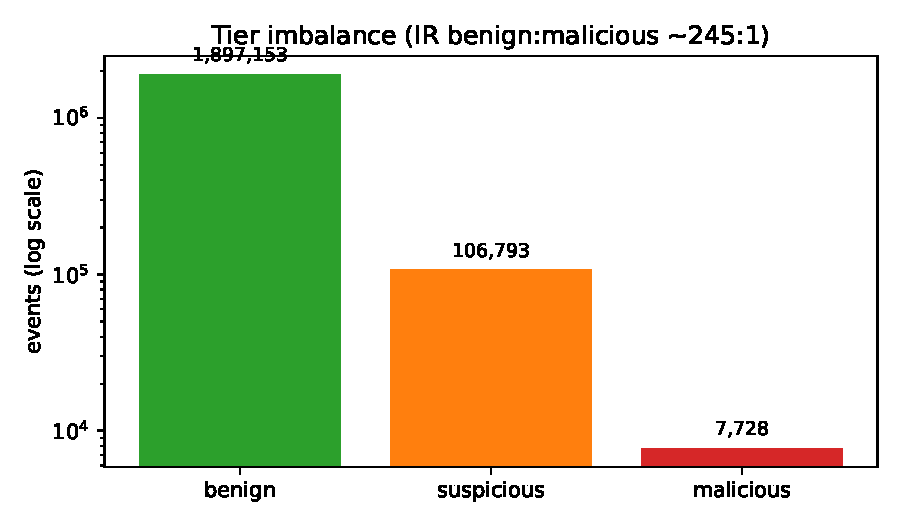
\includegraphics[width=\linewidth,height=.48\textheight,keepaspectratio]{label_distribution.pdf}

  \column{.49\textwidth}
  \centering
  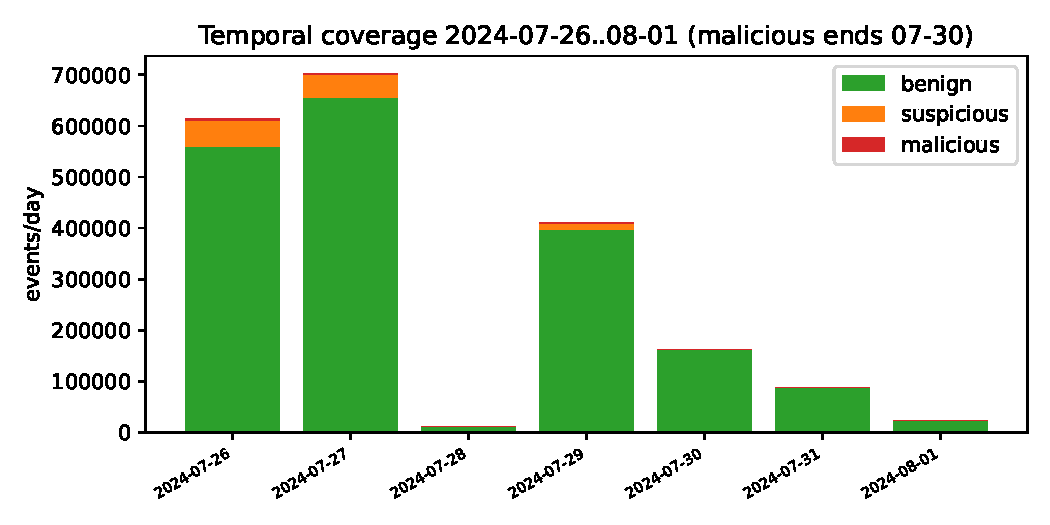
\includegraphics[width=\linewidth,height=.48\textheight,keepaspectratio]{temporal_volume.pdf}
\end{columns}
\vspace{0.15cm}
\small Malicious termina el 30 de julio; benign continúa al 1 de agosto. La prueba debe usar el futuro, no mezclar al azar eventos de una misma campaña.
\end{frame}

\begin{frame}{Las etiquetas son del motor, no del analista}
\begin{itemize}
  \item Precinct aplica \textbf{261 reglas lead}; las etiquetas del dataset vienen de esa correlación automática.
  \item \texttt{malicious}: lead de un incidente observado durante la ventana.
  \item \texttt{suspicious}: coincidencia con regla sin lead de incidente.
  \item \textbf{2,005,877 de 2,011,674} señales figuran como \texttt{Unprocessed}; no hay veredicto humano individual para casi todo el conjunto.
  \item MITRE ATT\&CK aporta lenguaje para conducta adversaria: táctica = objetivo, técnica = método. En estos datos, el mapeo ATT\&CK también deriva de reglas; se muestra como hint, no como verdad independiente.
\end{itemize}
\begin{alertblock}{Consecuencia}
  El sistema aprende cómo etiqueta Precinct. Su salida requiere contexto y revisión humana.
\end{alertblock}
\end{frame}

\section{Método y modelos}

\begin{frame}{Del evento a la consola del analista}
\centering
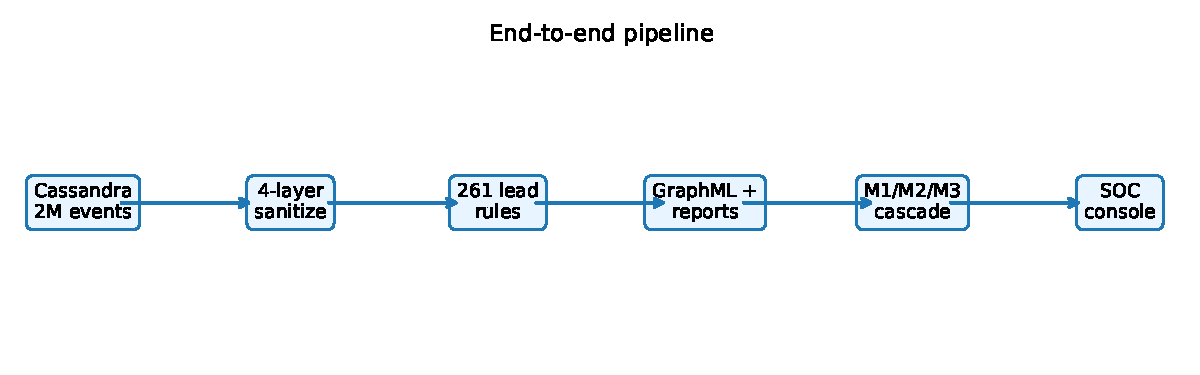
\includegraphics[width=.9\linewidth,height=.72\textheight,keepaspectratio]{architecture.pdf}
\vspace{0.1cm}

\small Vista conceptual. En la API final, \texttt{/score} fusiona M1+M2 y \texttt{/score\_graph} consulta M3 por separado.
\end{frame}

\begin{frame}{Tres vistas del mismo evento}
\begin{columns}[T,onlytextwidth]
  \column{.31\textwidth}
  \begin{block}{M1 · Tabular}
    Producto, acción, protocolo y hora. Base rápida para ordenar la cola.
  \end{block}
  \column{.31\textwidth}
  \begin{block}{M2 · Texto}
    Mensaje saneado con TF-IDF. Busca evidencia en el contenido del log.
  \end{block}
  \column{.31\textwidth}
  \begin{block}{M3 · Vecindario}
    Actividad previa de la misma organización, host o usuario.
  \end{block}
\end{columns}
\vspace{0.3cm}
\centering
Preprocesamiento: categorías con vacíos preservados · variables temporales · muestreo/pesos · TF-IDF · ocho estadísticas del vecindario.
\end{frame}

\begin{frame}{M1: rápido, pero casi no ve malicious}
\begin{columns}[T,onlytextwidth]
  \column{.54\textwidth}
  \begin{itemize}
    \item LightGBM, 200 árboles; categorías one-hot y 3 variables derivadas.
    \item Entrenamiento con muestra del pasado y pesos de clase; test futuro con prevalencia real.
    \item F1-macro \textbf{0.6276}; recall malicious \textbf{0.0107}.
    \item Recall suspicious \textbf{0.9885}: sirve como baseline/rankeador, no como detector de ataques raros.
  \end{itemize}
  \column{.42\textwidth}
  \centering
  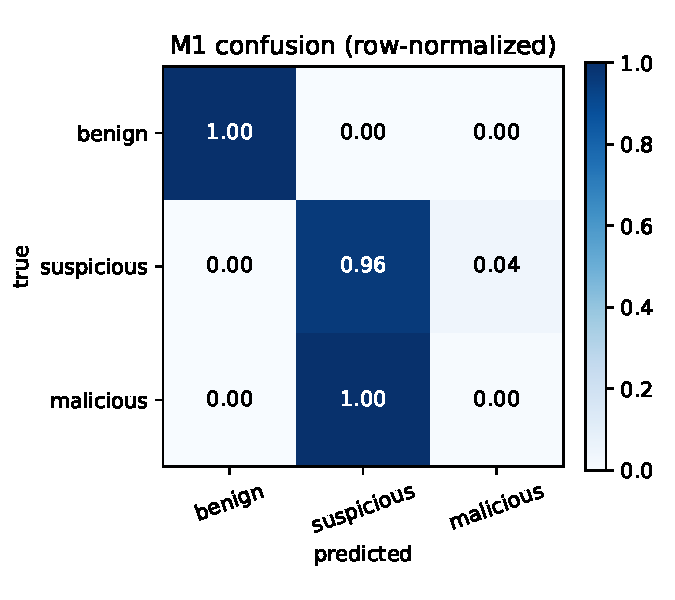
\includegraphics[width=\linewidth,height=.48\textheight,keepaspectratio]{confusion_m1.pdf}
\end{columns}
\end{frame}

\begin{frame}{M2: el texto aporta ranking, no dispara a umbral 0.5}
\begin{columns}[T,onlytextwidth]
  \column{.53\textwidth}
  \begin{itemize}
    \item TF-IDF de 5,000 términos + campos tabulares; XGBoost multiclass.
    \item F1-macro \textbf{0.6232}; recall malicious a umbral 0.5: \textbf{0.002}.
    \item PR-AUC malicious \textbf{0.218}; recall@1\%FPR \textbf{0.4344}.
    \item Conclusión: rescata ranking para revisión, pero no confirma por sí solo campañas futuras.
  \end{itemize}
  \column{.43\textwidth}
  \centering
  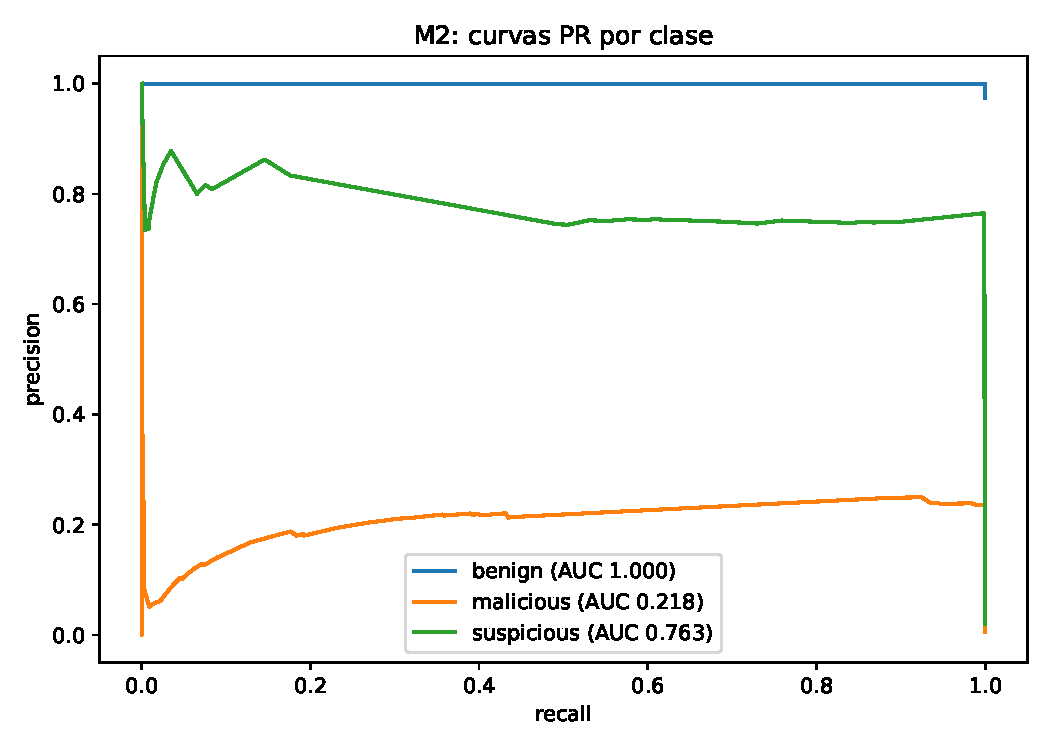
\includegraphics[width=\linewidth,height=.47\textheight,keepaspectratio]{pr_m2.pdf}
\end{columns}
\end{frame}

\begin{frame}{M3: una señal cambia al mirar sus vecinos}
\begin{columns}[T,onlytextwidth]
  \column{.52\textwidth}
  \begin{itemize}
    \item Ocho estadísticas de eventos previos que comparten host/IP/usuario en 300 s.
    \item Medición causal disponible: muestra balanceada de 10,656 eventos.
    \item F1-macro \textbf{0.6043}; malicious recall \textbf{0.99}; suspicious recall \textbf{0.07}.
    \item Complementa M2: cada vista recupera maliciosos que la otra omite.
  \end{itemize}
  \column{.44\textwidth}
  \begin{alertblock}{No confundir cifras}
    El 0.7186 del artefacto anterior usa ventana $\pm$5 min (incluye futuro): cota alta, no rendimiento causal del servicio.
  \end{alertblock}
\end{columns}
\end{frame}

\begin{frame}{Comparación: no hay un ganador único}
\centering
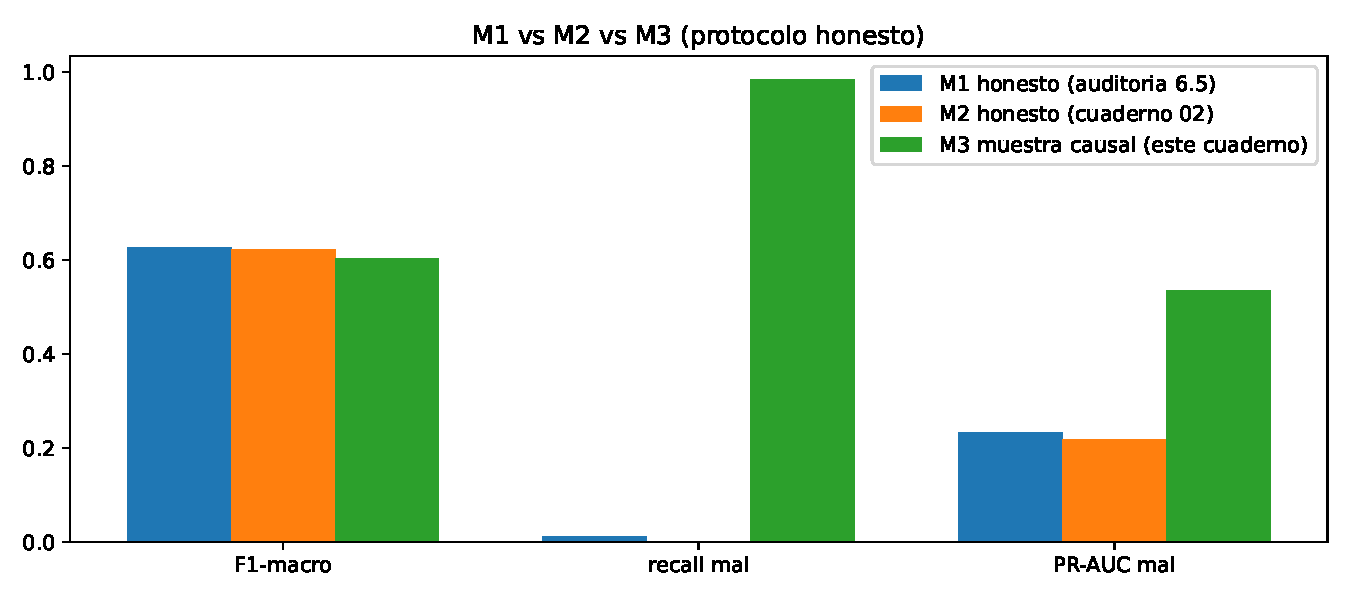
\includegraphics[width=.88\linewidth,height=.62\textheight,keepaspectratio]{compare_m123.pdf}

\small M1/M2 se evalúan en test poblacional; M3 causal, en test balanceado. Comparar por clase y protocolo, no solo por F1 global.
\end{frame}

\section{Ablaciones, límites y servicio}

\begin{frame}{ATT\&CK por evento: limitar lo que se promete}
\begin{itemize}
  \item M4a (LogReg) / M4b (XGBoost): seis técnicas; macro-F1 \textbf{0.252 / 0.256}.
  \item M4c tabular+grafo: macro-F1 \textbf{0.296}, pero con ventana $\pm$300 s no causal; T1041/T1567 siguen sin separarse.
  \item M4d por táctica: macro-F1 \textbf{0.426}; etiquetas frecuentes casi constantes inflan el promedio, las raras son débiles.
  \item M4t ajusta umbrales: macro-F1 tuned/fijo \textbf{0.354 / 0.354}; mueve recall/precisión, no crea información.
\end{itemize}
\begin{block}{Decisión de producto}
  La consola entrega ATT\&CK como hint derivado del tier/reglas, no como atribución aprendida confiable.
\end{block}
\end{frame}

\begin{frame}{Experimentos negativos que evitan sobreprometer}
\begin{columns}[T,onlytextwidth]
  \column{.48\textwidth}
  \begin{block}{M5 · Isolation Forest}
    Entrenado solo con benignos. Recall malicioso = 0; FPR benigno = 0.113; ROC-AUC = 0.174. El test es enriquecido (71.9\% amenaza), no prevalencia real; PR-AUC 0.724 está cerca de su baseline 0.719.
  \end{block}
  \column{.48\textwidth}
  \begin{block}{M6 · nivel incidente}
    Micro-F1 $\approx 1$ porque T1190/T1041/T1567 aparecen en los 9,688 incidentes de test. T1204 solo tiene 4 positivos.
  \end{block}
\end{columns}
\vspace{0.2cm}
\centering
Ninguno de los dos justifica automatizar detección o atribución.
\end{frame}

\begin{frame}{Qué se sirve y dónde queda el analista}
\begin{itemize}
  \item \texttt{POST /score}: M1 + M2; final malicious si cualquiera lo predice, si no conserva etiqueta M1.
  \item Regla operativa: escalar malicious o suspicious con acción \texttt{block}; en otro caso monitorear.
  \item \texttt{POST /score\_graph}: M3 por \texttt{artifact\_id}, consulta los 300 s previos y devuelve tier/probabilidades/número de vecinos.
  \item \texttt{GET /queue}, \texttt{/incident/\{id\}} y \texttt{/graph/vecindario}: cola, contexto de incidente y relaciones.
  \item Los modelos recomiendan prioridad; el analista valida evidencia y decide la respuesta.
\end{itemize}
\end{frame}

\begin{frame}{Demo en vivo · 3 minutos}
\begin{enumerate}
  \item Abrir la consola en \texttt{http://127.0.0.1:8000} y revisar la cola por riesgo.
  \item Abrir un incidente: leer reporte, señales relacionadas y cobertura ATT\&CK como hint.
  \item Enviar un evento a \texttt{/score}: ver M1, M2 y la decisión de triage.
  \item Consultar \texttt{/score\_graph} con un \texttt{artifact\_id}: mostrar vecinos de los 5 min previos.
\end{enumerate}
\begin{alertblock}{Si el servicio no está disponible}
  Usar las salidas guardadas de notebooks 02/03 y las figuras de \texttt{reports/figures/}; indicar que son resultados reproducibles, no una respuesta live.
\end{alertblock}
\end{frame}

\begin{frame}{Conclusión}
\begin{enumerate}
  \item El SOC necesita priorizar millones de señales con una fracción maliciosa muy pequeña.
  \item Campos, texto y contexto aportan evidencias distintas; M1/M2/M3 son complementarios, no solución autónoma.
  \item Las etiquetas son reglas de Precinct, hay deriva temporal y los resultados de ATT\&CK/M5/M6 no respaldan automatización.
  \item El producto correcto es una consola de apoyo al triage, con límites visibles y decisión final del analista.
\end{enumerate}
\vfill
\centering
\Large Preguntas
\end{frame}

\begin{frame}{Fuentes principales}
\small
\begin{itemize}
  \item WitFoo, \emph{Precinct6 Cybersecurity Dataset v2.1.0}, Apache-2.0.\\
    \url{https://huggingface.co/datasets/witfoo/precinct6-cybersecurity}
  \item WitFoo, \emph{dataset-from-precinct6}.\\
    \url{https://github.com/witfoo/dataset-from-precinct6}
  \item NIST SP 800-61 Rev. 3, \emph{Incident Response Recommendations and Considerations}.\\
    \url{https://csrc.nist.gov/pubs/sp/800/61/r3/final}
  \item MITRE ATT\&CK, FAQ: tácticas y técnicas.\\
    \url{https://attack.mitre.org/resources/faq}
  \item Resultados, métricas y limitaciones: \texttt{reports/paper.pdf}, \texttt{README.md} §5 y notebooks 00--10.
\end{itemize}
\end{frame}

\end{document}
